\documentclass[hyperref,french,usenames,xcolor=dvipsnames]{beamer}
 \mode<presentation>
{
\usepackage{beamerthemesplit}
\usetheme[compress,secheader]{Madrid}
%  \usecolortheme{orchid}
%	\setbeamercolor{alerted text}{fg=red!65!black}
  \setbeamercovered{transparent}
}

\usepackage{amsthm}
\usepackage{amsfonts}
\usepackage{amsmath}
\usepackage{graphicx}
%\usepackage{epsfig}
\usepackage{xspace}
\usepackage{stmaryrd}
%\usepackage{soul}
\usepackage[utf8]{inputenc}
%\usepackage[french]{algorithme}
%\usepackage[T1]{fontenc} %pour un beau PDF sous Linux ; à retirer sous Mac
\usepackage[french]{babel}

%\usepackage{ulem}
%\usepackage[english]{babel}
%\usepackage{times}
%\usepackage[utf8]{inputenc}
%\usepackage{amssymb}
%\usepackage{movie15}
%\usepackage{graphicx,color}
%\usepackage{hyperref}


%-----------------------------------------------------------

\definecolor{newcolor}{rgb}{0, 0, .90}
\definecolor{impcolor}{rgb}{.90, 0, 0}
\definecolor{darkergreen}{rgb}{0,0.5,0}
\definecolor{myorange}{rgb}{0.8,0.7,0}
\definecolor{myviolet}{rgb}{0.7,0.0,0.7}

\definecolor{lightpurple}{rgb}{0.83,0.27,1}
\definecolor{lightblue}{rgb}{0.27,0.9,0.9}



%\newcommand{\texthl}[1]{{\color{blue}#1}}
%\newcommand{\jaune}[1]{{\color{blue}#1}}
%\newcommand{\texthlb}[1]{{\color{orange}#1}}
%\newcommand{\orange}[1]{{\color{orange}#1}}
%\newcommand{\verte}[1]{{\color{green}#1}}
%\newcommand{\trad}{{\color{orange}{\bf $\leadsto$}}}

%\newcommand{\textcite}[1]{{\color{lightpurple}[#1]}}
%\newcommand{\textciten}[1]{{\color{lightpurple}#1}}

\newcommand{\texthl}[1]{{\color{red}#1}}
\newcommand{\jaune}[1]{{\color{red}#1}}
\newcommand{\texthlb}[1]{{\color{orange}#1}}
\newcommand{\orange}[1]{{\color{orange}#1}}
\newcommand{\verte}[1]{{\color{green}#1}}
\newcommand{\trad}{{\color{orange}{\bf $\leadsto$}}}

\newcommand{\textcite}[1]{{\color{myviolet}[#1]}}
\newcommand{\textciten}[1]{{\color{myviolet}#1}}

\newcommand{\montilde}{$\sim$}


\def \PH {\mathcal{PH}}
\def \PHb {\overline{\PH}}
\def \Hits {\mathcal{H}}
\def \GRN {\mathcal{G}}
\newcommand{\hitp}[2]{\mbox{$#1\rightarrow#2$}}
\newcommand{\hitb}[2]{\mbox{$#1\Rsh#2$}}
\newcommand{\hits}[3]{\mbox{$#1\xrightarrow{#3}#2$}}
\newcommand{\hitpath}[4]{\mbox{$#2\xrightarrow{#1}^*#3\Rsh#4$}}
\newcommand{\hit}[3]{\mbox{$#1\rightarrow#2\Rsh#3$}}

\title[REX MarkUs]%
{Contribution des Etudiants de l'Ecole Centrale de Nantes à Markus, un projet
libre.}

%\subtitle{Applications aux réseaux de Petri temporels et aux automates
%  temporisés}

\author[M. \textsc{Magnin}, G. \textsc{Moreau}, N. \textsc{Varoquaux}, B. \textsc{Vialle}]%
{Morgan \textsc{Magnin}, Guillaume \textsc{Moreau}, Nelle \textsc{Varoquaux} et Benjamin \textsc{Vialle}
}
\institute[ECN]{
\structure{
École Centrale de Nantes}
}

\date[14/07/2011]{Rencontres Mondiales du Logiciel Libre - 14/07/11}

%\date[] % (optional)
%{}

\subject{Rencontres Mondiales du Logiciel Libre - 14/07/11}

\AtBeginSection[] % Do nothing for \section*
{
\frame<beamer>
	{
	\frametitle{Sommaire}
	\tableofcontents[current]
	}
}

\begin{document}

\frame{\titlepage}

\section*{L'Ecole Centrale de Nantes et le Libre}

\frame
{
  \frametitle{Centrale Nantes}

  \begin{block}{École d'ingénieur généraliste}
    \begin{itemize}
      \item Compétences scientifiques et techniques
      \item Compétences humaines
      \begin{itemize}
	\item capacité à {\bf s'intégrer}
	\item capacité à {\bf communiquer}
	\item capacité à {\bf partager}
      \end{itemize}
    \end{itemize}
  \end{block}
  \begin{alertblock}{}
    Participation d'étudiants à des projets libres
  \end{alertblock}
}

\frame{
  \frametitle{En parallèle, un besoin...}
  {\bf Comment gérer et évaluer efficacement les travaux des étudiants en
  TP/Projet ?}
  \begin{itemize}
    \item Enseignants
    \begin{itemize}
      \item Gros volume de soumissions à traiter (plusieurs centaines par TP)
      \item Problématique d'harmonisation des notes entre groupes et correcteur
      \item Retour des corrections aux étudiants
    \end{itemize}
    \item Etudiants
    \begin{itemize}
      \item Comment récupérer les TP corrigés?
    \end{itemize}
  \end{itemize}
}

\frame{
  \frametitle{Le workflow actuel}
  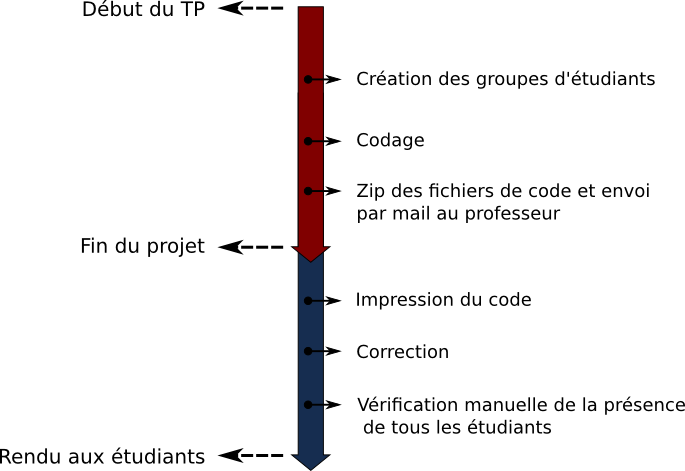
\includegraphics[scale=0.50]{images/WF-projet-avant.png}
  \begin{center}
  \end{center}
}


\frame{
  \frametitle{Markus, un outil de correction en ligne de travaux étudiant}
  \begin{itemize}
    \item Application Web
    \item Destiné à l'évaluation de projet informatique
    \item Dépôt versionné des travaux étudiants
  \end{itemize}
}


\section{Markus à Centrale Nantes}
\frame{
  \begin{itemize}
    \item 4 développeurs principaux
    \item Equipe trimiestrielle d'étudiant
  \end{itemize}

  \begin{itemize}
    \item Turnover des developpeurs très important
    \item difficulté pour maintenir une équipe stable qui comprenne la
    totalité du code
    \item Projet non communeautaire, mais dirigé par les demandes des clients
    et les projets étudiants
  \end{itemize}
}

\frame{
  \begin{itemize
}

\frame{
  \frametitle{Un projet étudiant type à Centrale Nantes}

  \begin{itemize}
    \item Ecriture d'un cahier des charges
    \item Implémentation de fonctionnalité
    \item Redaction de rapport hebdomadaire
    \item Réunion hebdomadaire(?) avec l'encadrant
    \item Rédaction d'un rapport final
    \item Présentation de 20min
  \end{itemize}
}

\frame{
\frametitle{Un projet étudiant type sur Markus}

  \begin{center}
  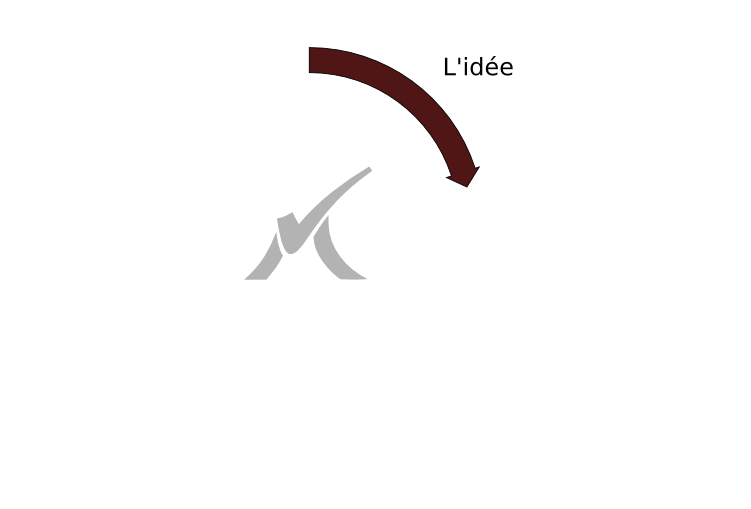
\includegraphics[scale=0.50]{images/markus-projet-etudiant_01.png}
  \end{center}
}

\frame{
  \frametitle{Un projet étudiant type sur Markus}
  \begin{center}
  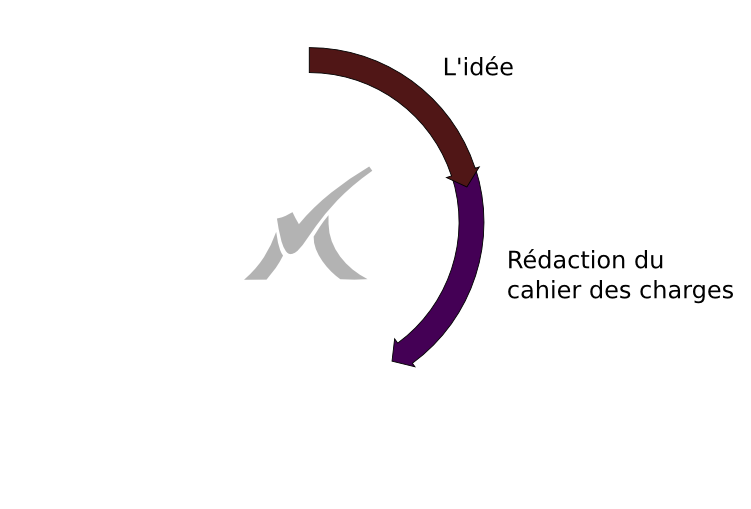
\includegraphics[scale=0.50]{images/markus-projet-etudiant_02.png}
  \end{center}
}

\frame{
  \frametitle{Un projet étudiant type sur Markus}
  \begin{center}
  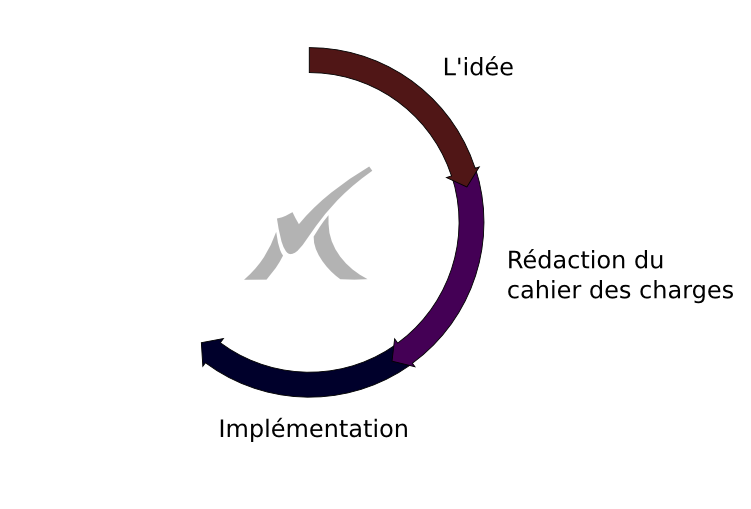
\includegraphics[scale=0.50]{images/markus-projet-etudiant_03.png}
  \end{center}
}

\frame{
  \frametitle{Un projet étudiant type sur Markus}
  \begin{center}
  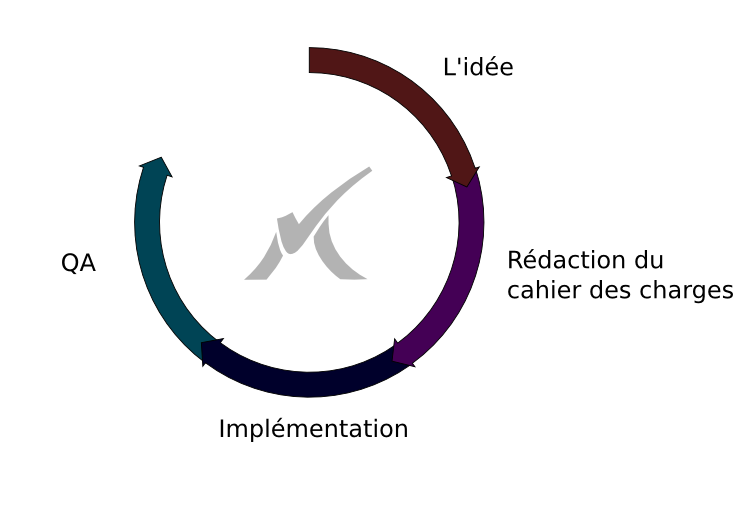
\includegraphics[scale=0.50]{images/markus-projet-etudiant_04.png}
  \end{center}
}

%\frame{
%  \frametitle{Un projet étudiant type sur Markus}
%  \begin{itemize}
%    \item Tests unitaites et fonctionnels
%    \item Revues de code
%  \end{itemize}
%  \begin{block}{}
%    Processus long
%  \end{block}
%}

\frame{
  \frametitle{Un projet étudiant type sur Markus}
  \begin{center}
  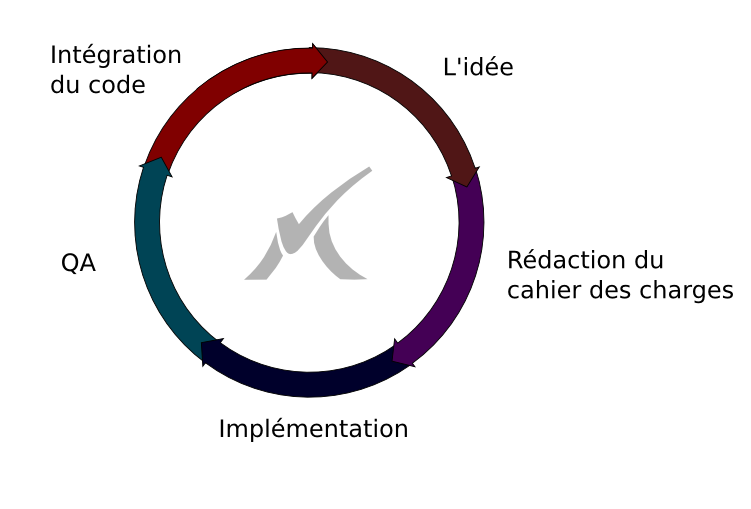
\includegraphics[scale=0.50]{images/markus-projet-etudiant_05.png}
  \end{center}
}

\frame{
  \frametitle{difficulté des étudiants}
  \begin{itemize}
    \item Projet complex:
    \begin{itemize}
      \item Rails, Ant, git etc...
      \item 15k de ligne de code
      \item présence non physique des mentors techniques
      \item Assurance qualité très strict
    \end{itemize}
  \end{itemize}
  \begin{block}{}
    Il est difficile d'avoir un patch intégré à la fin du projet.
  \end{block}
}

\section*{Conclusion}

\frame{
  \frametitle{Conclusion}

  Listes des fonctionnalités implémentées par des étudiants ECN dans Markus:
  \begin{itemize}
    \item Gestion des groupes - invitation des étudiants (Nelle Varoquaux)
    \item Refonte de l'interface utilisateur (Nelle Varoquaux)
    \item Framework de test (Benjamin Vialle)
    \item Implémentation des sections (Nelle Varoquaux \& Christian Jacques)
    \item Internationalisation \& traduction en français (Benjamin Vialle)
    \item Ajout d'un module d'annotation tactile (Clément delafargue, Benjamin Vialle
	  etc) \emph{en cours}
    \item Ajout d'un module d'annotation de formule mathématiques (Anthony Le
	  Jalle \& Mickael Lumbroso) \emph{en cours}
    \item Ajout d'un module de détection de plagiat (Shion Kashimura \& Benjamin
	  Thorrent) \emph{en cours}
    \item Migration à rails 3 (Benjamin Vialle) \emph{en cours}
  \end{itemize}

}

%\bibliography{biblio}

% http://eat-tice.ec-nantes.fr/wp-content/uploads/2011/06/magnin-moreau-QPES2011.pdf

%\bibliographystyle{alpha}

\end{document}
